\chapter{Initial Requirements}

\subsection{Introduction}
In this project we will create a SDN controller for defense against DDoS attacks. Through a REST API system, a web server can notify the begin of a DDoS attack; the controller will create an address change mechanism from D to D’.

\subsection{Implementation}
In this project we will implement:
%%%%AIUTO NON MI PRENDE L'IMMAGINE NON SO COME FARE NE CON ../images/ ne con images/
\begin{figure}[H]
\begin{center}
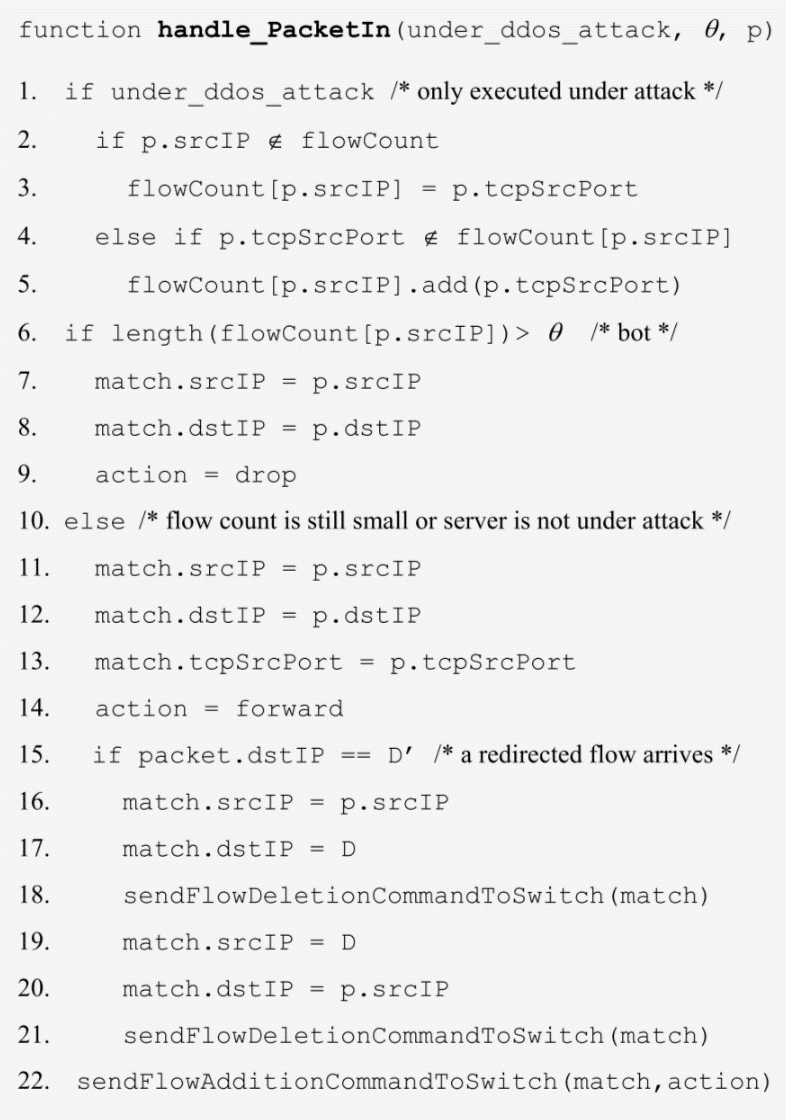
\includegraphics[]{images/PseudoCode.png}
\label{fig:pseudocode}
\caption{Pseudo code}
\end{center}
\end{figure}

We will implement a module inside ddosdefence-floodlight-controller/src/main/java/net/floodlightcontroller/ddosdefence here, there will be tree file: DDoSDefence.java, EnableDefenceResource.java IDDoSDefenceREST.java.

\subsection{Assumption}
Before starting the project we have thought about the issues we would have met, so we made the following assumption:
\begin{itemize}
	\item First part of the paper, which establishes the change of server address from D to D ', will not be implemented.
	\item Number of IP addresses: predefined and sufficient for the purpose of the project. Our project involves the management of the number of IP addresses via a circular list for assignment. 
	\item Our project plans to define a reCAPTCHA service: we will insert an equivalent implemented by us. *
	\item ARP Handling 
		\begin{itemize}
			\item Change the IP address but not the ARP table, the server will auto-assign the new IP address.
			\item This behavior is implemented in the forwarding module that must be included.
		\end{itemize}
	\item DELETE management: delete the precise rule dictated by the code. If you want to delete more than one, we must manage it keeping track of previous entries or inserting a maximum priority rule that invalidates the others.
\end{itemize}
* Assumptions are optional and will be implemented according to the difficulties we will encounter in the project.

\subsection{Testing System}
Our module will be tested using a set of scripts that we will produce, that emulates the client and server. Mininet will be used to create a virtual network composed  by a server and multiple (N) clients.

Server (h1) can use addresses from a /24 subnet, in our case 7.7.7.0/24 will be used.
Each client (h2-hN) will use an addresses took from the 80.80.80.0/24 subnet.
The Controller will listen for OpenFlow $PACKET_IN$ connections on 127.0.0.1:6653.
One OpenFlow switch (s1) will be used to connect all the previous entities. No routing or complex forwarding rules are required because the switch will solve the problem only using L2 Table packet switching. The only rule to use on both server and clients is \\
%\begin{lstlisting} %%%mi da errore sempre!!! uffffffff
“route add -net 0.0.0.0/32 dev <out interface>”
%\end{lstlisting}
\\
to send all the packet originated from the emulated device through the interface connected to the switch. ARP on the originating packet device will make sure to set the correct destination MAC address.
Clients can be regular service users or malicious ones:
\begin{itemize}
	\item Bots: will continuously do HTTP requests to a single target, but will not be able to compute any complex forwarding (like CAPTCHA or JavaScript implemented),
	\item Clients: will perform regular HTTP requests and be able to do forwarding.
\end{itemize}	
Both behaviours will be simulated using two separate scripts. Pseudo-code examples could be:
%\paragraph{./start_bot.sh serverip}
%\begin{lstlisting}
%While(true) {
	Establish HTTP on server connection using keepalive; exits when connection is closed
%}
%\end{lstlisting}
%\paragraph{./start_client.sh serverip}
%\begin{lstlisting}
%while(true) {
	%Establish HTTP on server connection using keepalive; exits when connection is closed
	%serverip = (if forwarded)  ? newaddress : serverip ; $#$ user can process forward
	%sleep 2; $#$ user will generate less traffic than bots
%}

%\end{lstlisting}

As stated on the paper, the forwarding method must be sufficiently complex to not be executed by the bots. However this represents an issue to $./start_client.sh$ script that is, in reality, a bot itself. To overcome this issue, we can initially simplify the forwarding mechanism to let the script do the forward. However the $./start_bot.sh$ will ignore, in good faith, the simplified forwarding directive.
An example of HTTP Page forwarding response could be one not containing an HTML page (we can check if contains <html> or not) but containing the address to forward. This is just for a testing purpose and can be subjected to changes due to chosen web server implementation.

\begin{figure}[H]
\begin{center}
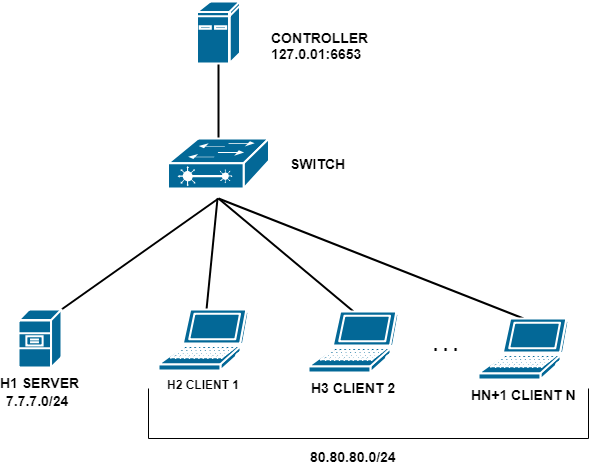
\includegraphics[]{images/TestingTopology.png}
\label{fig:testing}
\caption{Testing Topology}
\end{center}
\end{figure}

\paragraph{Checking the correct behaviour for OpenFlow rules:} 
mininet> dpctl dump-flows
This command can be used to dump all the switch flow entries.

\subsubsection{Testing Parameters}
%%%%%DA SISTEMARE%%%%
%Timeout ? (quello nel codice di anto)
%\tehta = attack flow entry count threshold
%Cmax = number of maximum allowable connections
%Cattack = number of attack signaling connections
%n = number of legitimate users
%k = number of  bots
%\lamba norm - average request arrival rate from legitimate users
%\lamba attack - average request arrival rate from bots
%\mu service rate

\subsection{Final Documentation and Reporting}
At the end of this project will be produced:
\begin{itemize}
	\item Final report: accompanying document illustrating the choices made and the reasons for these choices for the implementation of the module,
	\item Summary presentation in which the work carried out will be shown,
	\item Demo to show how the module works.
\end{itemize}
